\appendixpageoff % Eliminar la página introductoria a apéndices

\begin{appendices}
\chapter{Microcontrolador}
\section{Resolver problemas de memoria\label{memFlash}}
A lo largo del desarrollo del firmware, será necesaria la gestión de
áreas de memoria reservadas para ciertas funcionalidades, por ejemplo
en el bloque de configuración del firmware, \textit{setup()}; será
necesario reservar un área en memoria para las labores de E/S y memoria
intermedia de las acciones con tensor.

Para ello se contará con la propia \textit{flash}
del dispositivo a modo de región de almacenamiento. Creando arrays en la
propia memoria \textit{flash} que harán las veces de mecanismo de
almacenamiento como se expone en el siguiente fragmento de código:\\

\begin{lstlisting}[firstnumber=62,title=Fragmento de \textit{deep\_pen.ino}]
    /************************ SETUP FUNCTION ************************/
    // Setting the area of memory reserved to tensor input-output actions.
    constexpr int TensorAreaSize = 30 * 1024;
    uint8_t tensor_arena[TensorAreaSize];
\end{lstlisting}


\section{Instalación de librerías en \textit{Arduino IDE}\label{libArduino}}
La instalación de librerias es muy sencilla haciendo uso del
\textit{Arduino IDE}. En el menú: \textit{Tools}->\textit{Manage
Libraries...} y se abrirá una ventana donde podemos gestionar las
librerías instaladas, instalar otras versiones e instalar nuevas
librerías.


\section{Notificación de conexión \textit{Bluetooth} del firmware
del microcontrolador\label{BTcon}}
Para solucionar el problema de la notificación de conexión \textit{Bluetooth}
se crea una pequeña estructura para consultar el estado de conexión de la iteración
anterior (\textit{last\_connection}). De esta forma es posible mantener consistencia
en la conexión pese a estar dentro de un bucle.


\section{Definición de micro-operaciones en el firmware del
microcontrolador\label{firmwMO}}
Las micro-operaciones que se definirán en el firmware que
se emplearán en la red neuronal son:
\begin{itemize}
    \itemsep0em 
    \item Conv2: Para el procesamiento de la capa homónima.
    \item Mean: Para promedios como el que se necesita en la capa \textit{GlobalAveragePooling2D}
    \item FullyConnected: Para las capas densas, entre otros.
    \item SoftMax: Como función de activación.
\end{itemize}

Como alternativa más cómoda, pero a costa de un mayor uso de memoria,
del cual no podemos abusar dada la naturaleza de nuestro dispositivo;
es plausible usar \textit{tflite::AllOpsResolver}, que cargará todas las
operaciones disponibles para \textit{TFLite}.


\section{Cambiar la orientación de la placa}
Para poder hacer uso del \textit{SmartPen} en una posición de escritura natural,
vertica, hay que hacer una serie de cambios.
Los mejores resultados se han conseguido cambiando en la biblioteca de los sensores,
en LSM9DS1.cpp en todas los sensores:
\begin{lstlisting}[firstnumber=121,language=c++,title=Fragmento
    de \textit{LSM9DS1.cpp} de la librería homónima]
//          Original         //     Orientacion cambiada
x = data[0] * 4.0 / 32768.0; // z = -data[0] * 4.0 / 32768.0;
y = data[1] * 4.0 / 32768.0; // y =  data[1] * 4.0 / 32768.0;
z = data[2] * 4.0 / 32768.0; // x =  data[2] * 4.0 / 32768.0;
\end{lstlisting}

Aunque continúan sin obtenerse trazados correctos del movimiento.


\chapter{Red neuronal}
\section{Ajuste para poder utilizar el recolector de muestras de \textit{Pete Warden}\label{PWchrome}}
Es necesario hacer uso del recolector de muestras, utilizar \textit{Google Chrome}
y activar la flag para desarrolladores '\textit{Experimental Web Platform features}'
activa en '\textit{chrome://flags/}'\textsuperscript{\cite{petewardenmw}}.


\section{Asignación incorrecta de índices en el recolector de muestras\label{borraIndices}}
Como se ha citado en el \textit{apéndice \ref{borrarMuestras}} anterior,
al borrar muestras se borran más trazos de los debidos y eso genera
una redistribución de los índices de cada muestra, resultando incorrectos.

Para resolverlo, se ha creado un script que reasigna los índices con
la distribución adecuada: 
\href{https://github.com/AntonioPriego/SmartPen/blob/main/Utils/sort_dataset.py}{sort\_dataset.py}


\section{El recolector de muestras elimina varias muestras al borrar una\label{borrarMuestras}}
Este fallo aparentemente se produce al borrar instancias por debajo de
la última. En ocasiones, se produce un pequeño error en las comprobaciones
de índices de muestras, por lo que se borran varias muestras y estas terminan
con índices desordenados.

Para paliar este problema y comprobar si había el número de trazos esperado,
se hacía uso de un comando en bash cada vez que se generara un \textit{JSON}:

\begin{lstlisting}[language=bash]
    ~$ grep -o index <nombre_archivo>.json | wc -l
\end{lstlisting}


\section{Descripción de capas \textit{Keras} empleadas para la implementación
de la red neuronal\label{capasKeras}}

Las capas utilizadas durante la implementación del modelo,
son las siguientes\textsuperscript{\cite{keras}}:
\begin{itemize}
    \itemsep0em 
    \item Rescaling: Como resultado de esta capa,
    se consigue reescalar o normalizar
    los valores de los inputs, en nuestro caso las imágenes. Con esto definimos
    una escala uniforme y es un procedimiento típico en procesamiento de imagen:
    \textit{image normalization}, donde se normalizará el valor de los píxeles
    de las imágenes a una escala [0,1].
    \item Conv2D: Capa para procesamiento convolucional,
    es la capa que realmente
    procesará dentro del modelo. Se crea un kernel que convoluciona con la entrada
    de la capa. Se define la capa en base ciertos parámetros que determinarán su
    funcionamiento y complejidad, siendo en nuestro caso los parámetros:
    \begin{itemize}
        \itemsep0em 
        \item filters: el número de filtros de salida de la convolución.
        \item kernel\_size: el tamaño de ventana de convolución, cuando se
        especifica un solo número, se interpreta una ventana cuadrada de ese
        tamaño.
        \item strides: define el tamaño de los tramos de salto de la ventana
        de convolución.
        \item input\_shape: establecer el tamaño de la entrada. En nuestro caso
        imágenes de 32x32.
    \end{itemize}
    \item BatchNormalization: Normaliza sus entradas por lotes.
    Aplica transformaciones
    que conservan la media de la salida cercana a 0 y la desviación estándar a 1.
    \item Activation: aplica una función de activación a una salida. Las funciones de
    activación son las que arbitran la activación de las neuronas de la red neuronal
    y por ello, repercute en su salida. Existen diversas
    funciones de activación, como lo son \textit{rectified linear unit(relu)},
    \textit{sigmoid}, \textit{softmax}(función de distribución de probabilidad), etc.
    \item Dropout: Capa que introduce cierta entropía, de forma que se descarta
    la contribución de ciertas neuronas de forma estadística. Se suelen implementar
    para soslayar el \textit{overfitting}.
    \item GlobalAveragePooling2D: Esta capa tomará un
    tensor de dimensión $x*y*z$ y
    calculando el valor medio de los valores $x$ e $y$, producirá una salida basada en
    $z$ elementos.
    \item Dense: Es una capa común de red neuronal,
    solo que está \textit{densamente}
    conectada, es decir, cada neurona de esta capa está conectada a todas las neuronas
    de la capa anterior. Se usa, como es nuestro caso, en redes clasificatorias.
\end{itemize}

\begin{figure}[]
    \centering
    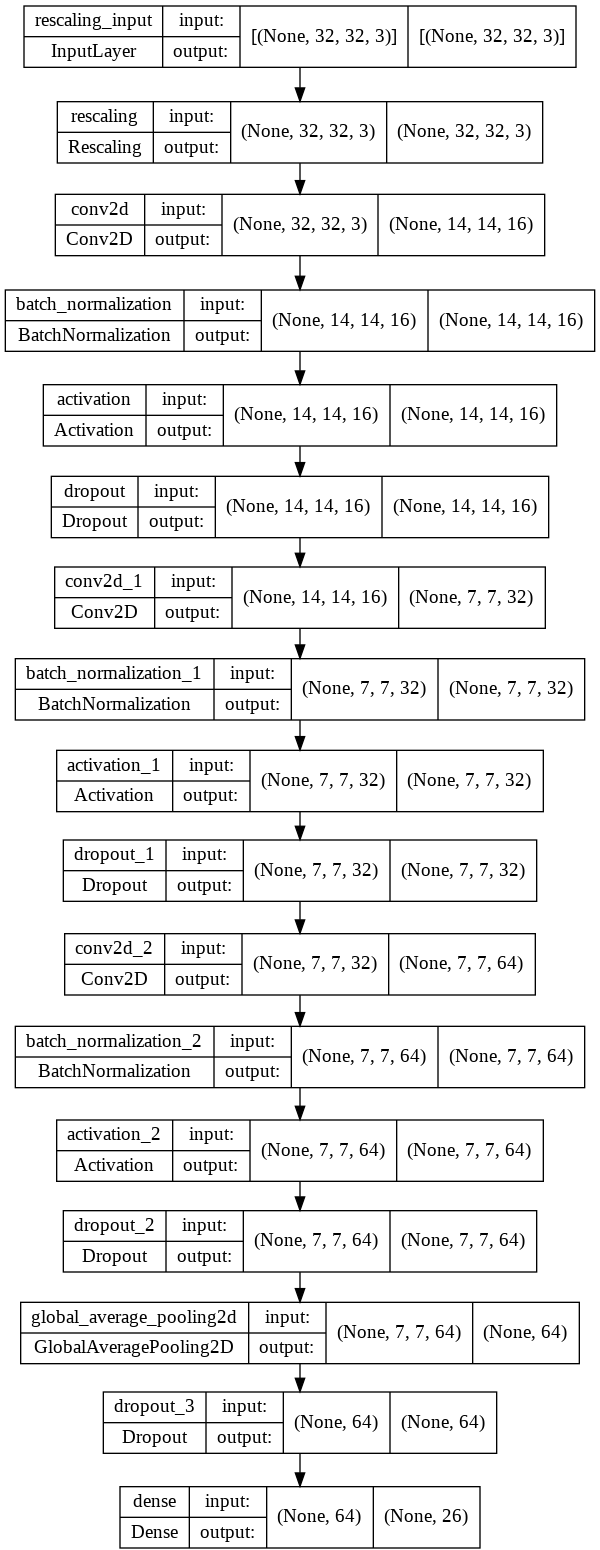
\includegraphics[width=0.69\textwidth]{capturas/estructuraRNTF.png}\\[-0,2cm]
    \caption{Estructura del modelo generado en \textit{TensorFlow}\label{estRN}}
\end{figure}

La anterior \textit{figura \ref{estRN}} es consecuencia del siguiente código:
\begin{lstlisting}[language=python, title=Fragmento de \href{https://github.com/AntonioPriego/SmartPen/blob/main/Train/Train.ipynb}{\textit{Train.ipynb}}]
################# MAKING THE MODEL ###############

def make_model(input_shape, num_classes):
    model = models.Sequential()

    # Rescaling
    model.add( layers.Rescaling(1.0 / 255) )
    # Block 1
    model.add( layers.Conv2D(16, 5, strides=2, input_shape=input_shape) )
    model.add( layers.BatchNormalization() )
    model.add( layers.Activation("relu") )
    model.add( layers.Dropout(0.45) )
    # Block 2
    model.add( layers.Conv2D(32, 5, strides=2, padding="same") )
    model.add( layers.BatchNormalization() )
    model.add( layers.Activation("relu") )
    model.add( layers.Dropout(0.45) )
    # Block 3
    model.add( layers.Conv2D(64, 3, strides=1, padding="same") )
    model.add( layers.BatchNormalization() )
    model.add( layers.Activation("relu") )
    model.add( layers.Dropout(0.45) )
    # Pooling + another Dropout
    model.add( layers.GlobalAveragePooling2D() )
    model.add( layers.Dropout(0.45) )
    # Softmax
    model.add( layers.Dense(num_classes, activation="softmax") )


    return model

model = make_model(input_shape=(IMAGE_WIDTH, IMAGE_HEIGHT, 3),
                        num_classes=NUM_CLASSES)
model.build(input_shape=(None, IMAGE_WIDTH, IMAGE_HEIGHT, 3))
model.summary()
keras.utils.plot_model(model, show_shapes=True)
\end{lstlisting}

\section{Experimentación red neuronal}
\subsection{Estructura de la red neuronal\label{expRN}}
Cada uno de los modelos o cambios con los que se ha experimentado, son
pequeñas iteraciones o pequeñas variaciones respecto del modelo base.
Creado a partir del estudio de otros modelos para tareas parecidas.

Una de las abundantes variables con las que experimentar, es el
tamaño de las imágenes de entrada para la red neuronal. Se ha
percibido una notoria mejora en el reconocimiento con letras
complejas, como por ejemplo la 'k', a medida que las dimensiones aumentan. 
De forma análoga, con letras simples, como por ejemplo la 'c', a razón de
una menor resolución, mejores resultados se obtenían. Esto cuadra con lo
esperable, ya que las letras complejas necesitan de un análisis más preciso
para obtener mejores predicciones que el resto y equivalentemente, las letras
más sencillas obtienen mejores predicciones sobre el resto, cuando se analizan
muestras sencillas.

También se ha estudiado el comportamiento del tamaño del \textit{kernel} en
las capas \textit{Conv2D}. Se ha experimentado para tamaños (cuadrados) de entre 3 a 5, ya
que menos resultaría poco conveniente y más sería desproporcionado teniendo en
cuenta que trabajamos con información espacial igual o inferior a 32x32.
En general se ha observado que a mayor tamaño de kernel, se obtiene una mayor
precisión en el testeo y si siente al probar el modelo, que funciona ligeramente
mejor. A costa evidentemente de una mayor complejidad del modelo y por tanto
de un mayor tamaño en memoria. Por lo que se ha optado por mantener en el
modelo final tamaño de \textit{kernel} 5x5 en los dos primeros bloques de \textit{convolución}
y de 3x3 en el último, ya que a esta capa llega información de dimensiones mucho menores
(7x7). Sin embargo, la decisión de aumentar la complejidad del modelo, también
implica aumentar el número de \textit{epochs} en la etapa de entrenamiento, para
desentrañar mejor el comportamiento más adecuado de una estructura más compleja,
aunque esto se tratará en la siguiente sección.

Otro parámetro que se ha analizado es el número de bloques de convolución (explicados
en la Sección \ref{disenioRN}), con solo dos, los resultados no son nada buenos, y
añadiendo un cuarto, se obtienen resultados muy buenos pero concretamente en algunas
letras hay clasificaciones erróneas, posiblemente debido a \textit{overfitting}
(concepto introducido en Teoría \ref{ovYun}) y se obtienen buenos resultados en general,
pero no suficientes para una buena experiencia.

Se experimentó con la capa \textit{BatchNormalization} de los bloques de convolución.
Al eliminar esta capa de los bloques, se obtienen en fase de testeo, clasificaciones
correctas, pero con una precisión mucho menor, llegando a alcanzar en algunos casos,
la mitad de precisión que con el modelo base. Como cabía esperar, la normalización de
las entradas resulta muy útil para mejorar la precisión, y aunque no se aprecie en
el testeo, también proporciona un entrenamiento más rápido.

Con el resto de capas del bloque de convolución, no se ha experimentado, porque
son capas manifiestamente indispensables.

Aunque si bien, sí que se ha experimentado con los valores de \textit{Dropout}, estudiándolos
para valores de $0.4$ a $0.6$, ya que para el resto de valores, resulta un \textit{dropout}
demasiado restrictivo o demasiado laxo. Obteniendo los mejores resultados para 0.45, aunque
si bien, las diferencias eran prácticamente indistinguibles durante su uso.

\subsection{Entrenamiento de la red neuronal\label{expTrainRN}}
En esta fase, los cambios siguen siendo muy relevantes para el desempeño de la red neuronal,
sin embargo hay menos parámetros que estudiar.

Yo me he centrado principalmente en las \textit{epochs} y el \textit{learning rate}, aunque
también he probado someramente los \textit{optimizadores}.
Las \textit{epochs} son las iteraciones que se darán en el algoritmo de entrenamiento.
A más epochs, mayor será la profundidad en el entrenamiento.
Esto no quiere decir que si empleamos el doble de \textit{epochs}, consigamos el doble
de precisión, no es un fenómeno lineal, sino que el modelo presenta un techo
alcanzable y por más que se entrene, no van a obtenerse mejores resultados. Por lo que
la clave es encontrar un número de \textit{epochs} que resulte en un buen entrenamiento,
pero sin emplear tiempo de más. En nuestro caso, para los modelos experimentales más complejos,
se ha empleado un número mayor de \textit{epochs}, pero en general, ningún modelo ha seguido
presentando mejoras notorias más allá de las 100 \textit{epochs}. Por tanto, se usará este valor.

El segundo parámetro de estudio, ha sido el \textit{learning rate}, que simplificándolo,
sería el valor que determina el progreso de entrenamiento que se hace en cada \textit{epoch}.
Un \textit{learning rate} más alto, se traduce en un entrenamiento que escala mejor con pocas
\textit{epochs}, pero que está más limitado a alcanzar el resultado óptimo del modelo;
análogamente, un \textit{learning rate} más bajo, resulta en un entrenamiento que
escalará peor, pero que puede alcanzar un resultado potencial mejor, como ilustra la Figura \ref{lRate}.
En nuestro caso se ha experimentado con valores de \textit{learning rate} entre $0.00095$ y $0.0015$
ya que en muchos modelos estudiados y parecidos a este, se usa un valor cercano a $0.001$.
y como nuestro modelo no es muy complejo, podemos permitirnos un escalado menor, ya que no llevará
mucho tiempo entrenar al modelo y hay margen para aumentarlo sin problema. Por lo que
nos quedamos con un \textit{learning rate} de $0.00095$.

Respecto a los \textit{optimizadores}, se ha experimentado muy laxamente, así que para asegurar,
nos quedamos con el \textit{optimizador} de referencia del modelo base.

\begin{figure}[h]
    \centering
    \subfloat[\textit{learning rate 0.00095}]{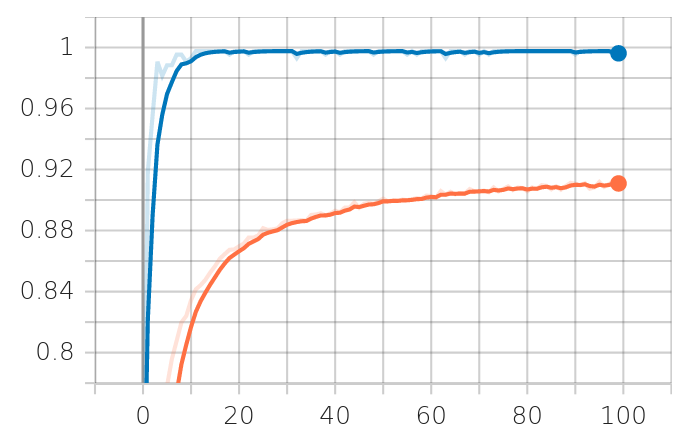
\includegraphics[width=0.45\textwidth]{capturas/accuracyMref.png}}
    \hfill
    \subfloat[\textit{learning rate 0.0015}]{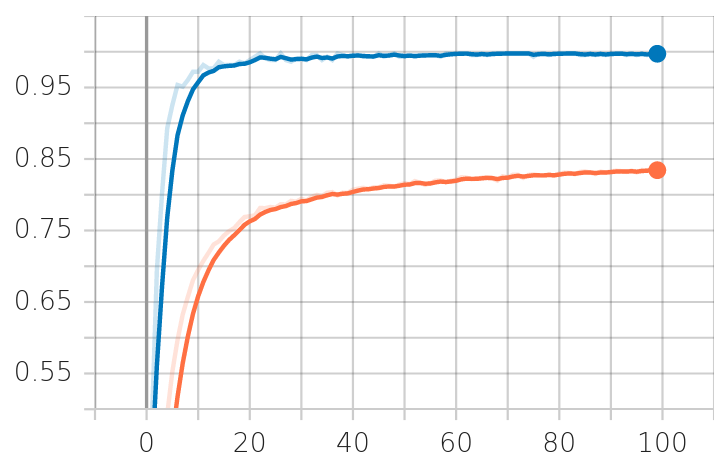
\includegraphics[width=0.45\textwidth]{capturas/accuracyMlrMayor.png}}
    \caption{Escalado de \textit{accuracy} por \textit{epochs}\label{lRate}}
\end{figure}
{\small {\color{cyan}Azul}: Validación | {\color{orange}Naranja}: Entrenamiento. Mismo modelo, distinto \textit{learning rate}.}

\chapter{Interfaz de usuario}
\section{Permisos uso del puerto del microcontrolador (Linux)\label{pserie}}
En algunos casos, como ocurrió en el trascurso de este trabajo,
si queremos acceder al puerto serie de la placa o usar el IDE de
Arduino, debemos conceder permisos al microcontrolador:
\begin{lstlisting}[language=bash]
    ~$ ls -l /dev/ttyACM*                     # En mi caso
    ~$ sudo usermod -a -G dialout <usuario>
\end{lstlisting}

Como respuesta al error ``\textit{can't open device /dev/ttyACM0}''.


\section{Acceso al puerto serie en QT (Linux)\label{psQT}}
Hay que añadir al *.pro del proyecto QT:
\begin{lstlisting}[language=make]
  QT += serialport
\end{lstlisting}
Y tras esto, añadir la librería con normalidad y acceder al puerto
con el nombre, en nuestro caso, "ttyACM0".

\section{Valores nulos al leer por \textit{Bluetooth} con \textit{QT}}
Este fue un error complejo de depurar como suele ser habitual
con los problemas derivados de versiones de librerías. No se
leía ningún valor de las \textit{características} del dispositivo pese a estar detectándolas y estar
correctamente conectado, se debía a dos factores.

El primero estar haciendo uso de una librería anterior a la documentación con
la que estaba trabajando (librería de QLowEnergyService). Hay grandes diferencias
en el comportamiento de algunos métodos de esta librería de las versiones 5.x
a la 6.x, aunque estas no provocan errores, sí que provocan que el
el código no funcione como se esperaría (\textit{Enums} con valores diferentes o inexistentes, etc).


En segundo lugar se estaba llamando a un método cuando todavía no se había recibido
la \textit{característica}. Por tanto esta aparentaba estar bien registrada, ya que
podía obtenerse su \textit{Uuid}, pero no contenía ningún valor.
Se estaba leyendo el valor en \textit{connectToService()},
cuando debería hacerse en \textit{serviceDetailsDiscovered()}.


\section{Error de reconocimiento de imágenes en QT}
Al importar imágenes en QT tras haber exportado el programa a Win o Linux para
corroborar que todo continuara funcionando correctamente, las imágenes
dejaron de mostrarse.
Esto se debe a que QT cambia la ruta del proyecto al directorio en el que se
exporta el programa. Por tanto las rutas especificadas para las imágenes, dejan de ser
válidas. Para corregir este problema, basta con cambiar el '\textit{Build directory}'
del proyecto (Desde '\textit{Projects}' en el panel de la derecha de QT creator).


\section{Pérdida de valores de \textit{características}\label{errlibQTBT}}
Este es teóricamente el fix para las desconexiones aleatorias,
sin embargo en mi caso y en el de otros desarrolladores, no termina
de funcionar, si bien sí que permite no perder las características
durante las desconexiones. \cite{carBTQT}

Este parche hace que el código del callback de la librería, no asuma que
hay un periférico conectado, que es lo que presuntamente, provoca
la desconexión.

Debe editarse la librería \textit{QLowEnergyControllerPrivateBluezDBus}
con los cambios resaltados en el siguiente enlace:
\url{https://codereview.qt-project.org/c/qt/qtconnectivity/+/233087/3/src/bluetooth/qlowenergycontroller_bluezdbus.cpp#563}.

Pese a que no haya funcionado en mi caso, sí que ha sido muy importante
ya que ha corregido en parte un mal comportamiento de la librería.
Estas son las causas por las que es mucho mejor elegir herramientas
con una comunidad amplia y activa detrás.


\section{Error de permisos al lanzar la interfaz de usuario (Linux)\label{permBTQT}}
Al ejecutar el \textit{UI}, aparece este error en los logs:
'\textit{qt.bluetooth.bluez: Missing CAP\_NET\_ADMIN permission. Cannot determine whether a found address is of random or public type.}'
Para ello hay que modificar la configuración del \textit{dbus} y dotar de permisos
a nuestro usuario.\textsuperscript{\cite{permBTQT}}
\newpage
\begin{lstlisting}[language=bash]
<policy user="yourUserName">
    <allow own="org.bluez"/>
    <allow send_destination="org.bluez"/>
    <allow send_interface="org.bluez.Agent1"/>
    <allow send_interface="org.bluez.MediaEndpoint1"/>
    <allow send_interface="org.bluez.MediaPlayer1"/>
    <allow send_interface="org.bluez.Profile1"/>
    <allow send_interface="org.bluez.GattCharacteristic1"/>
    <allow send_interface="org.bluez.GattDescriptor1"/>
    <allow send_interface="org.bluez.LEAdvertisement1"/>
    <allow send_interface="org.freedesktop.DBus.ObjectManager"/>
    <allow send_interface="org.freedesktop.DBus.Properties"/>
</policy>
\end{lstlisting}

Si persiste el problema, otra forma de solucionarlo es mediante el comando:
\begin{lstlisting}[language=bash]
    sudo setcap CAP_NET_ADMIN=eip <path hasta el ejecutable>
\end{lstlisting}

\section{Capturas de la interfaz de usuario\label{ifazUsu}}
\begin{figure}[h]
    \centering
    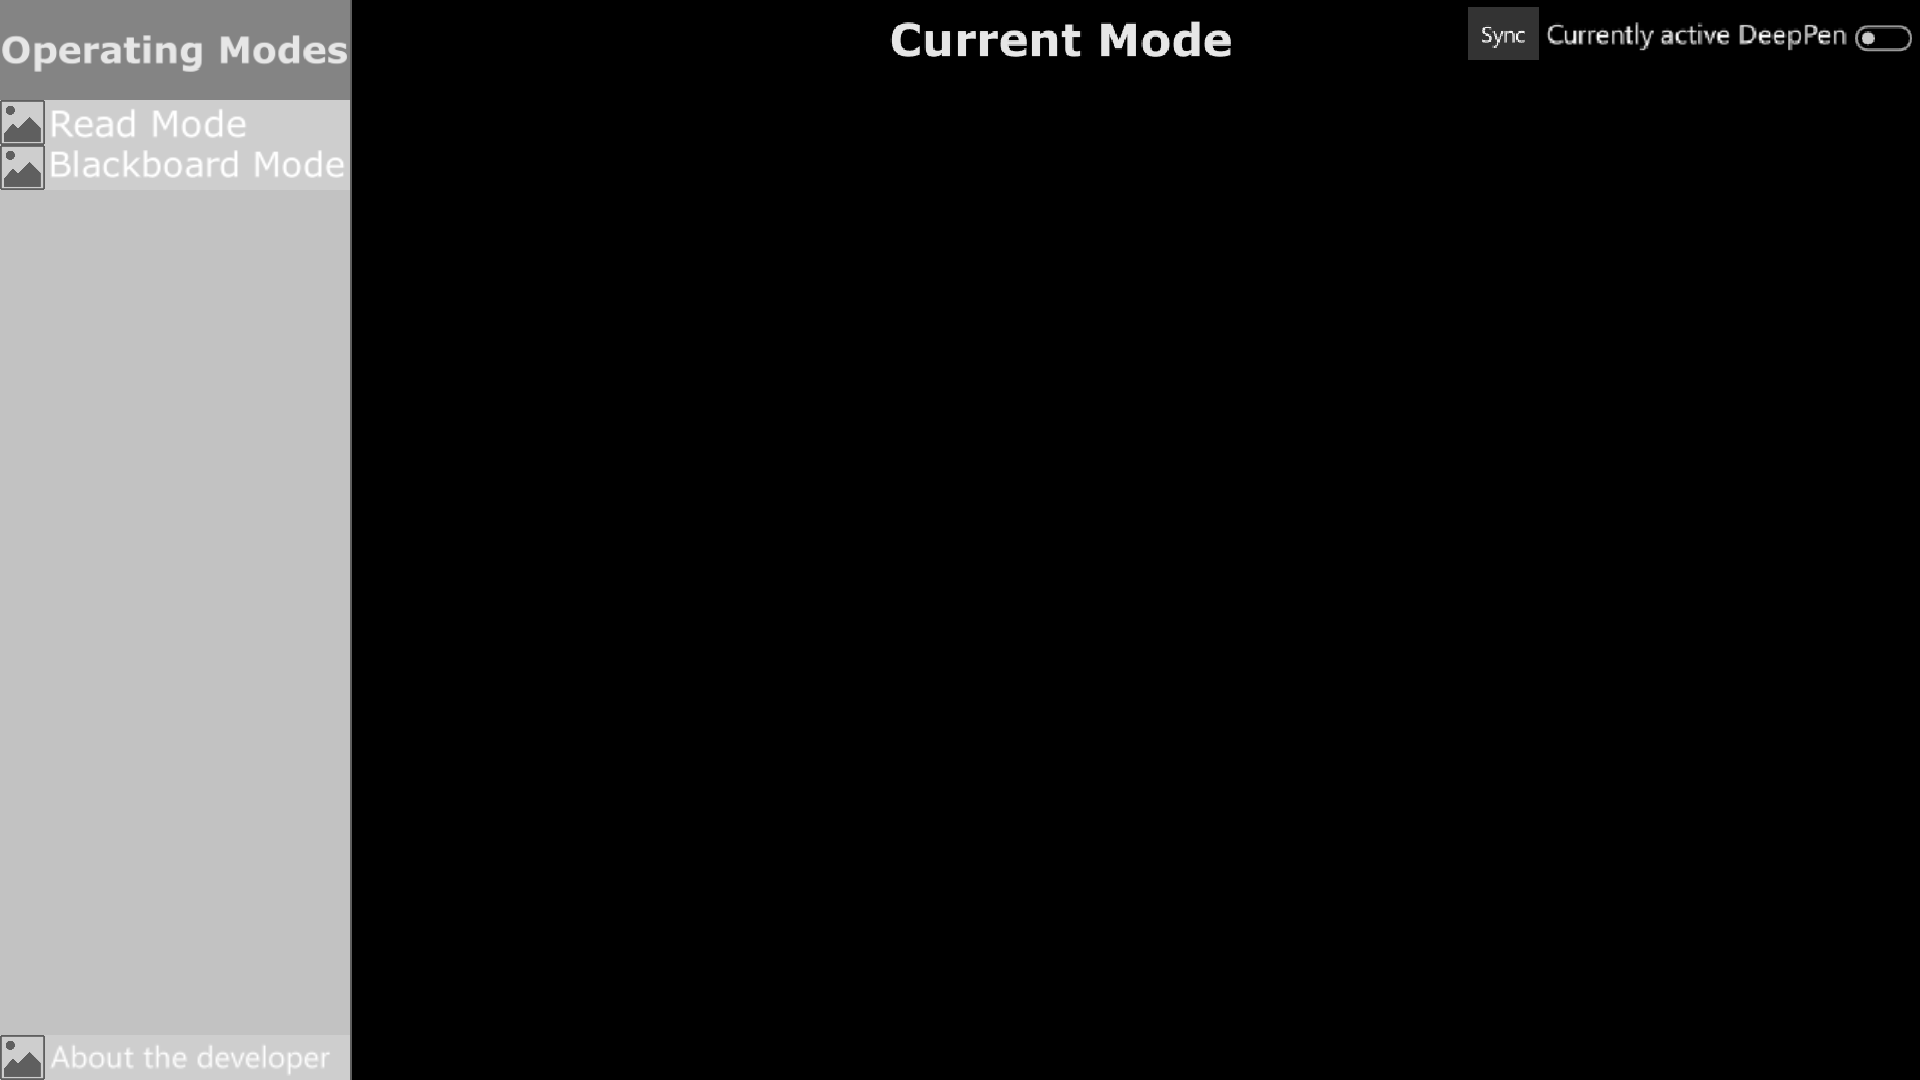
\includegraphics[angle=270,width=0.49\textwidth]{capturas/DisenoUsuario2.png}\\[-0,35cm]
    \caption{Boceto en QT Design Studio}
\end{figure}

\begin{figure}[h]
    \centering
    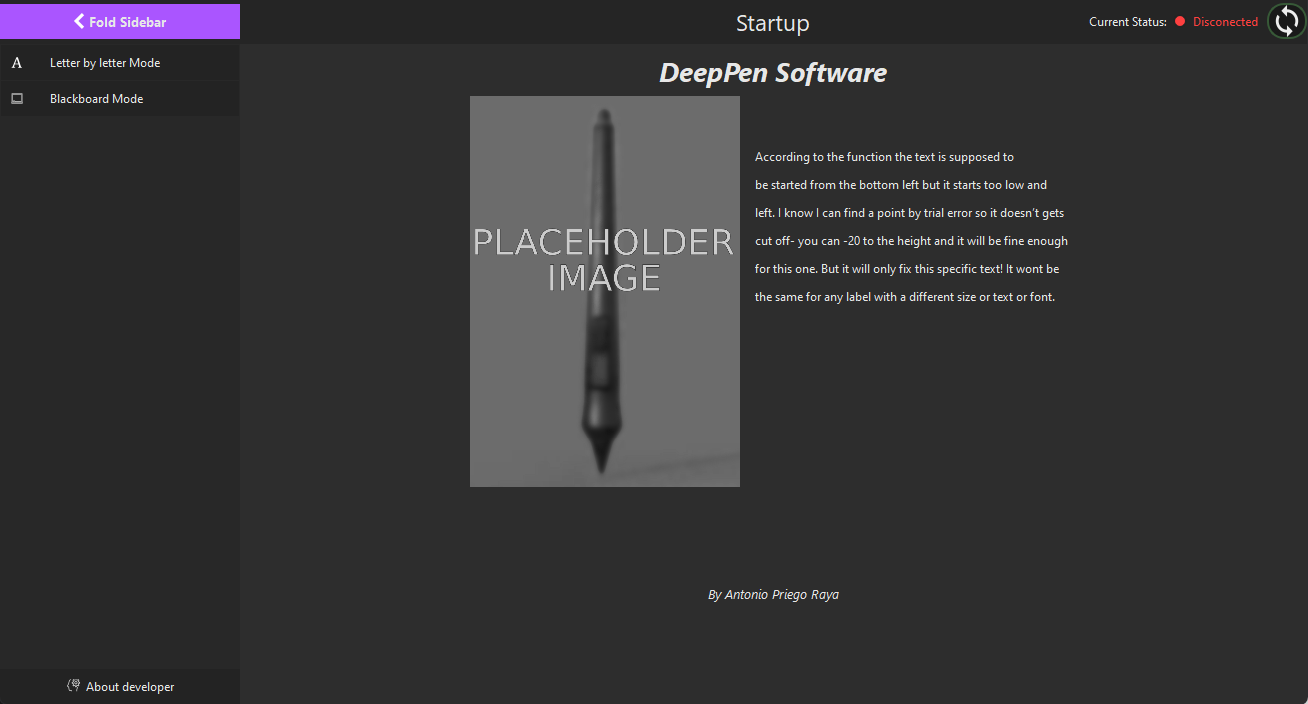
\includegraphics[angle=90,width=1\textwidth]{capturas/Interfaz.png}\\[-0,35cm]
    \caption{Resultado de la implementación de la interfaz de usuario}
\end{figure}

\chapter{Encapsulado}
\section{Modelos 3D\label{modelos}}
\begin{figure}[h]
    \centering
    \subfloat[\href{https://github.com/AntonioPriego/SmartPen/tree/main/SmartPenModel/Components/cilindroAlto}{cilindroAlto}]{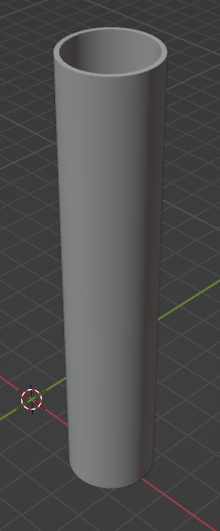
\includegraphics[width=0.185\textwidth]{capturas/cilindroAlto.png}}
    \hfill
    \subfloat[\href{https://github.com/AntonioPriego/SmartPen/tree/main/SmartPenModel/Components/slotBateria}{slotBateria}]{\includegraphics[width=0.405\textwidth]{capturas/slotBatería.png}}
    \hfill
    \subfloat[\href{https://github.com/AntonioPriego/SmartPen/tree/main/SmartPenModel/Components/cilindroBajo}{cilindroBajo}]{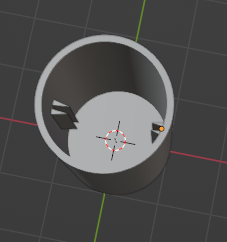
\includegraphics[width=0.4\textwidth]{capturas/cilindroBajo.png}}
    \caption{Componentes útiles del encapsulado}
\end{figure}

  \begin{figure}[h]
    \centering
    \subfloat[\href{https://github.com/AntonioPriego/SmartPen/tree/main/SmartPenModel/Components/clip}{clip}]{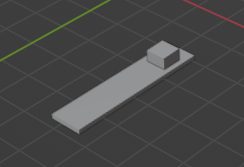
\includegraphics[width=0.27\textwidth]{capturas/clip.png}}
    \hfill
    \subfloat[\href{https://github.com/AntonioPriego/SmartPen/tree/main/SmartPenModel/Components/punta}{punta}]{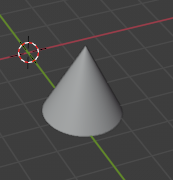
\includegraphics[width=0.18\textwidth]{capturas/punta.png}}
    \hfill
    \subfloat[\href{https://github.com/AntonioPriego/SmartPen/tree/main/SmartPenModel/Components/semiEsfera}{semiEsfera}]{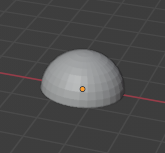
\includegraphics[width=0.21\textwidth]{capturas/semiEsfera.png}}
    \caption{Decoración del encapsulado}
  \end{figure}

\section{Resultado de integrar todo en el encapsulado\label{encapsulado}}
\begin{figure}[h]
    \centering
    \subfloat[SmartPen vista frontal]{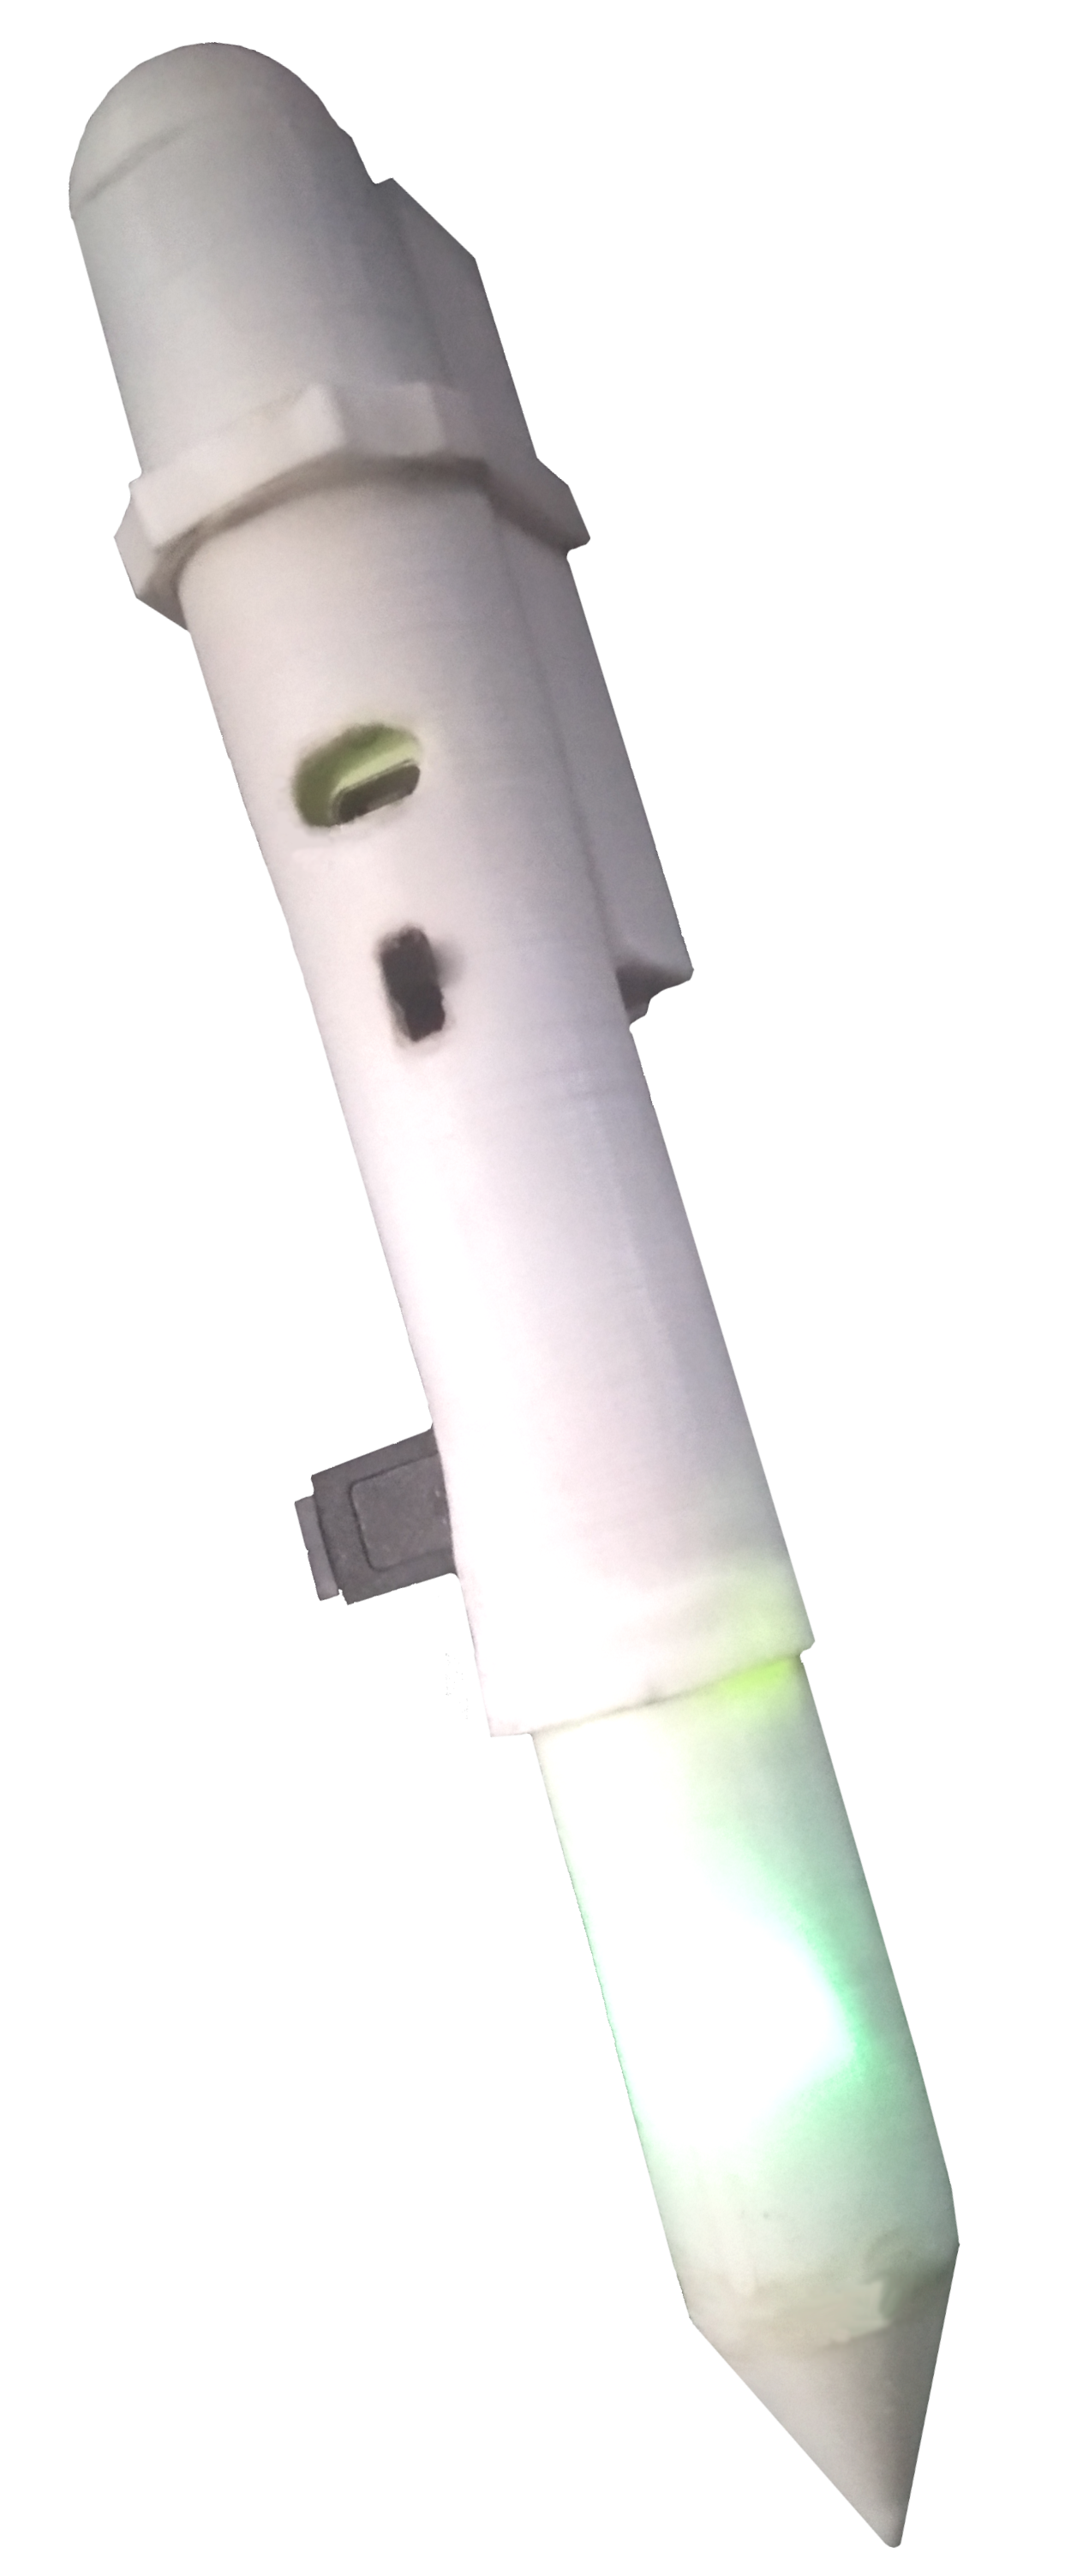
\includegraphics[width=0.48\textwidth]{capturas/SmartPen.png}}
    \hfill
    \subfloat[SmartPen vista trasera]{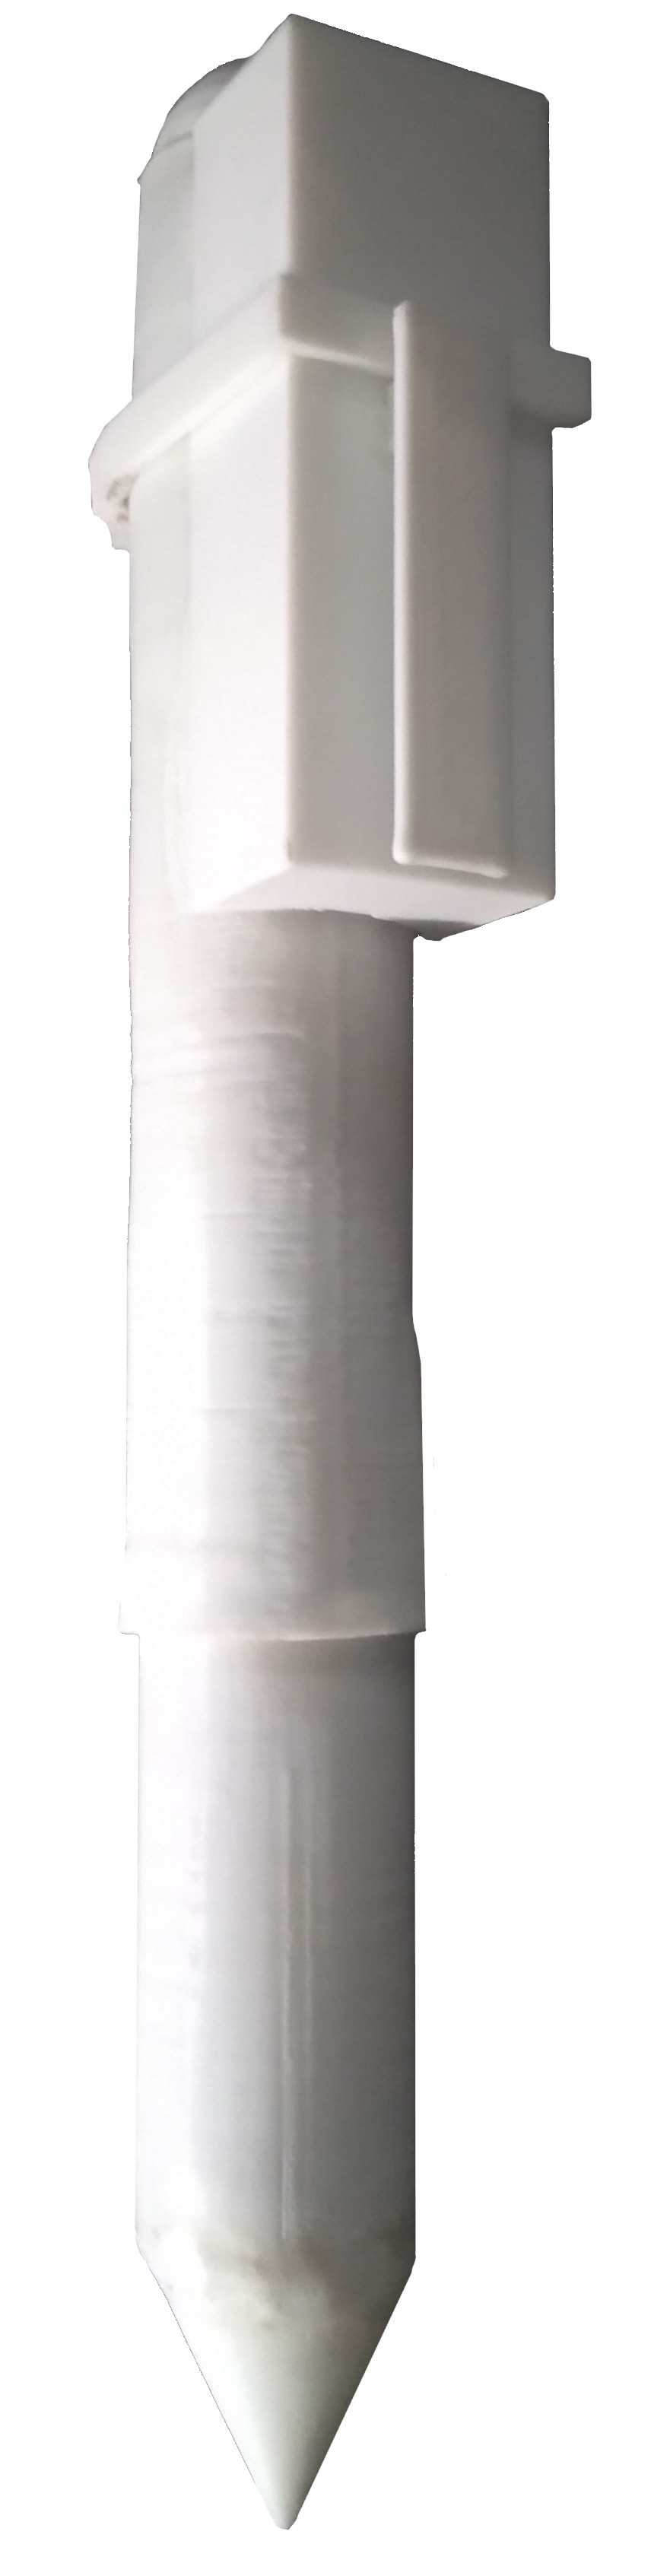
\includegraphics[width=0.29\textwidth]{capturas/SmartPenTrasero.png}}
    \caption{SmartPen}
  \end{figure}

\end{appendices}